\documentclass[12pt, a4paper]{article}

\usepackage[utf8]{inputenc}

% Limit the page margin to only 1 inch.
\usepackage[margin=1in]{geometry}

%Imports biblatex package
\usepackage[
backend=biber,
style=alphabetic
]{biblatex}
\addbibresource{../math-342w.bib}

% Enables the `align' environment.
\usepackage{amsmath}
\allowdisplaybreaks
\usepackage{bm}
\usepackage{array}
\usepackage{rotating}
\usepackage{multirow}

% Provides useful environments, such as:
% - \begin{proof} ...\end{proof}
\usepackage{amsthm}
\newtheorem{proposition}{Proposition}
\theoremstyle{definition}
\newtheorem*{definition}{Definition}
\newtheorem{theorem}{Theorem}
\newtheorem{corollary}{Corollary}
\newtheorem*{example}{Example}
\newtheorem{algorithm}{Algorithm}

% Enables using \mathbb{}, for example \mathbb{N} for the set of natural numbers.
\usepackage{amssymb}

% Allows using letters in enumerate list environment. Use, for example:
%\begin{enumerate}[label=(\alph*)]
% ...
%\end{enumerate}
\usepackage[inline]{enumitem}

% Enable importing external graphic files and provides useful commands, like \graphicspath{}
\usepackage{graphicx}
% Images are located in a directory called "images" in the current directory.
\graphicspath{{./images/}}

% Make links look better by default.
% See: https://tex.stackexchange.com/questions/823/remove-ugly-borders-around-clickable-cross-references-and-hyperlinks
\usepackage[hidelinks]{hyperref}
\usepackage{xcolor}
\hypersetup{
	colorlinks,
	linkcolor={red!50!black},
	citecolor={blue!50!black},
	urlcolor={blue!80!black}
}

% Code Listings. Source:
% https://stackoverflow.com/questions/3175105/inserting-code-in-this-latex-document-with-indentation
\usepackage{listings}
\usepackage{color}
\usepackage[most]{tcolorbox}

\definecolor{dkgreen}{rgb}{0,0.6,0}
\definecolor{gray}{rgb}{0.5,0.5,0.5}
\definecolor{mauve}{rgb}{0.58,0,0.82}

\lstset{frame=tb,
	language=Java,
	aboveskip=3mm,
	belowskip=3mm,
	showstringspaces=false,
	columns=flexible,
	basicstyle={\small\ttfamily},
	numbers=none,
	numberstyle=\tiny\color{gray},
	keywordstyle=\color{blue},
	commentstyle=\color{dkgreen},
	stringstyle=\color{mauve},
	breaklines=true,
	breakatwhitespace=true,
	tabsize=3
}

\title{Lecture 23: MATH 342W: Introduction to Data Science and Machine Learning}
\author{Sergio E. Garcia Tapia\thanks{Based on lectures of Dr. Adam Kapelner at Queens College.
See also the \href{https://github.com/kapelner/QC_MATH_342W_Spring_2025}{course GitHub page}.}}
\date{May 6th, 2025 (last updated \today)}

\begin{document}
	\maketitle
	\section{Bagging for Classification}
	Recall that in the context of regression, we defined $g_{\text{avg}}$ by
	\begin{align*}
		g_{\text{avg}} := \frac{g_1 + g_2 + \cdots + g_M}{M}
	\end{align*}
	where $g_i$ are fit on different bootstrap samples to get more independence
	and drive down the variance term in the Bias-Variance Trade-off. If
	$\mathcal{Y}$ is categorical, then we define $g_{\text{avg}}$ using
	the \text{mode}:
	\begin{align*}
		g_{\text{mode}} := \text{Mode}[g_1, g_2, \ldots,g_M]
	\end{align*}
	We did not talk about the Bias-Variance Trade-off in this context, but there
	is analogous theory, though more complicated and we will not go into it here.
	\section{Missingness in Future Units}
	Last time we talked about the need to perform imputation to deal with missingness
	in our data. Let's consider again what happens when we do a train-test split
	and there is missingness, as in Figure~\ref{fig:train-test-missing}.
	\begin{figure}
		\centering
		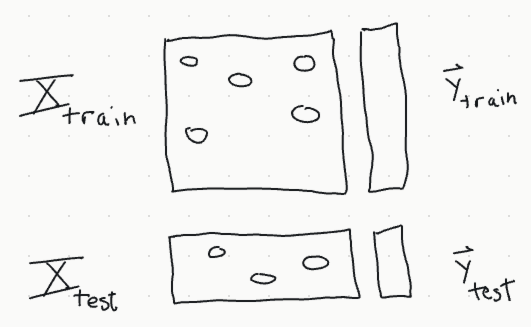
\includegraphics[width=0.4\textwidth]{train-test-split-missingness}
		\caption{Train-test split of a data set $\mathbb{D}$ that exhibits
		missingness.}
		\label{fig:train-test-missing}
	\end{figure}
	We want to construct binary matrix $M$ whose entries indicate missingness of entries
	in $X$, and then impute with the MissForest algorithm that we saw. However,
	we want to be careful not to look at $\bm{y}_{\text{test}}$ because it may
	influence our $g$, thereby increasing the risk that we are dishonest. Therefore,
	we make $\bm{y}_{\text{test}}$ entries all missing (in R, this means \texttt{NA}),
	and then we impute. The algorithm imputes the missing values for both $X_{\text{test}}$
	and $\bm{y}_{\text{test}}$, and we can discard the latter because not only do
	we already have them (we artificially made them missing for correctness), but
	these are the values we are predicting to begin with (the $\hat{\bm{y}}_{\text{test}}$
	we will compute).
	
	At the end of this, we will have computed a prediction function $g$:
	\begin{align*}
		g = \mathcal{A}(\langle [X_{\text{imp}}, M] , \bm{y} \rangle, \mathcal{H})
	\end{align*}
	
	So far, all of this has been review to tackle the following question:
	how do we predict in the future for a unit $\bm{x}_{*}$ exhibiting
	missingness? The short answer is that you cannot, and we must fill in
	the missingness. There are three approaches we can try:
	\begin{enumerate}[label=(\textbf{\arabic*})]
		\item \textbf{Recompute (slowest but most accurate)}: This means we impute
		$X_{\text{updated}}$, consisting of the $n$ rows of $X$ and $\bm{x}_*$ as row
		$n + 1$. Then we create a new predictive function:
		\begin{align*}
			g_{\text{updated}} = \mathcal{A}(\langle [X_{\text{imp, updated}}, M_{\text{updated}}] , \bm{y} \rangle, \mathcal{H})
		\end{align*}
		See Figure~\ref{fig:predicting-future-by-recomputing}.
		\begin{figure}
			\centering
			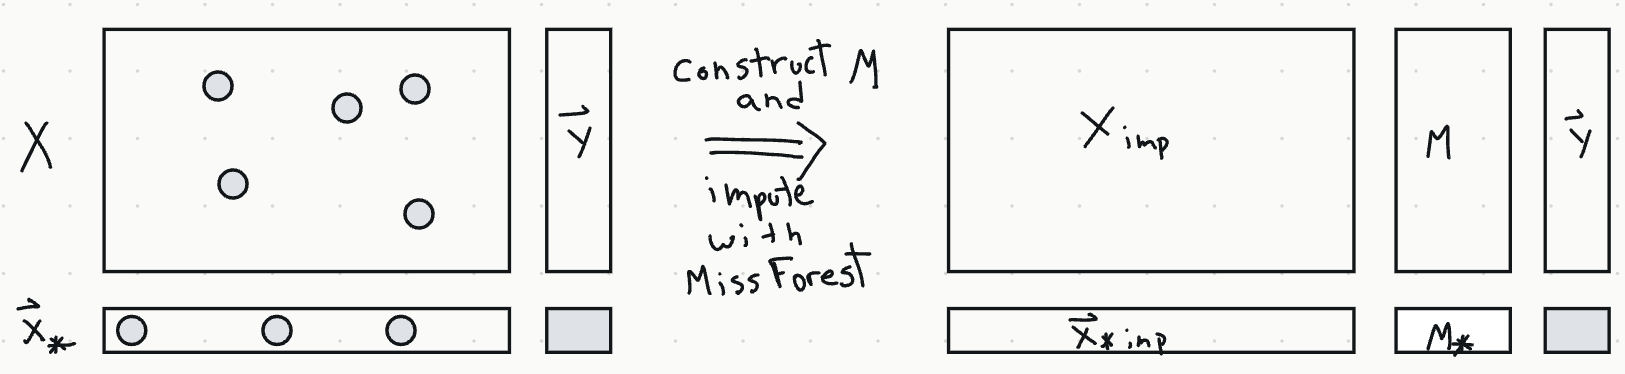
\includegraphics[width=1.0\textwidth]{predicting-future-unit-with-missingness-recomputing}
			\caption{Predicting on a future unit that has missingness by recomputing the entire model.}
			\label{fig:predicting-future-by-recomputing}
		\end{figure}
		Because we have more data, this may result in an improvement, but it can
		be expensive. This may be reasonable if we are doing batch predicting,
		meaning that we are predicting for much more than just one new unit.
		
		\item \textbf{Reuse (fastest but least accurate)}: In this case, we
		do not start the imputation from our original $X$. We start with
		$[X_{\text{imp}} \mid M]$, and we impute on the matrix with $n+1$ rows
		consisting of $[X_{\text{imp}} \mid M]$ and $[\bm{x}_* \mid M_*]$.
		Because there is only one row of missing data now, it is much faster.
		After imputing, thereby eliminating the missingness in $\bm{x}_*$,
		we use the \text{old} $g$ to predict:
		\begin{align*}
			\hat{\bm{y}} = g([\bm{x}_{*, \text{imp}} \mid M_*])
		\end{align*}
		\begin{figure}
			\centering
			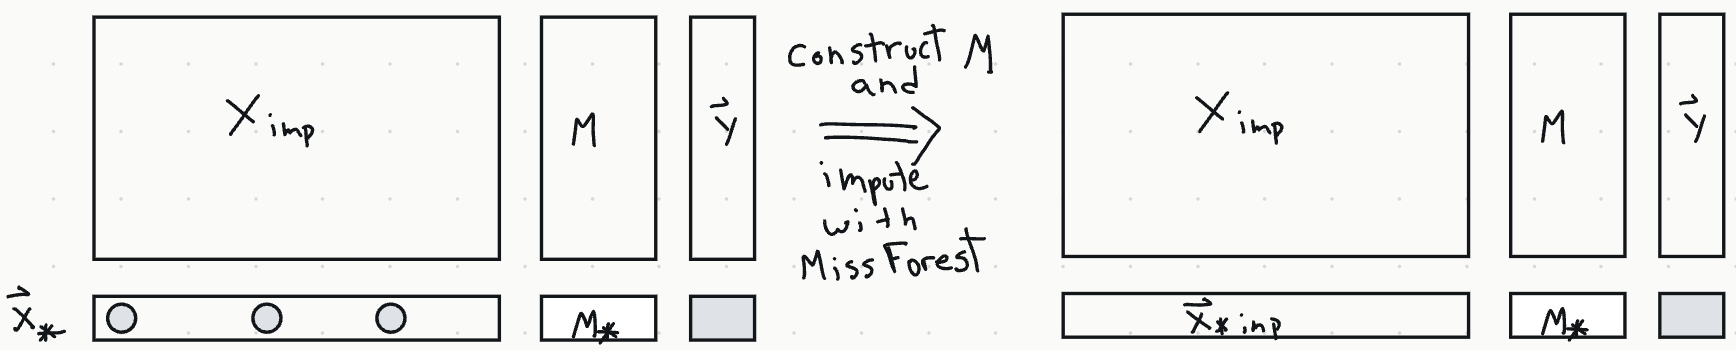
\includegraphics[width=1.0\textwidth]{predicting-future-unit-with-missingness-reuse}
			\caption{Predicting on a future unit that has missingness by reusing the existing model.}
			\label{fig:predicting-future-by-reuse}
		\end{figure}
		See Figure~\ref{fig:predicting-future-by-reuse}.
		
		\item \textbf{Middle strategy}: Do the imputation from (1), but do not
		refit $g$. Use the old $g$ to predict.
	\end{enumerate}
	\section{Probability Estimation in Asymmetric Cost Modeling}
	We saw that in a classification setting, we may need to distinguish between
	false positives and false negatives; they both correspond to mispredictions,
	but one may be more costly than the other. If $C_{FP}$ is the cost of
	false-positives, $C_{FN}$ is the cost of false negatives, and
	$C_{FP} > C_{FN}$ (say, $C_{FP}= 100 \cdot C_{FN})$, then we want to be
	absolutely sure that when we predict $\hat{y} = 1$, then it is indeed
	a true positive. How do we incorporate this heuristic in our model?
	
	For example, instead of using the \text{mode} (highest frequency), can
	we do something else? The canonical way to do this is with
	\textit{probability estimation}. We seek something of the form
	\begin{align*}
		\hat{p}_{*} = g(\bm{x}_*) \implies
		\hat{y}_{*} = \underset{\hat{p}_* \geq p_{\text{th}}}{\mathbb{I}}
	\end{align*}
	In other words, we predict the probability that a new unit $\bm{x}_*$
	corresponds to a true positive. If that probability exceeds a threshold
	$p_{\text{th}}$, then we predict positive for $\bm{x}_*$.
	The value $p_{\text{th}}$ is called the \textbf{probability threshold}
	and it is a hyperparameter. For example, it may be $50\%$. We want
	to be very sure that when we say $\hat{y} = 1$, it is indeed the case
	that $y = 1$ since $C_{\text{FP}}$ is so high. As $C_{FP}$ increases,
	we may want to increase $p_{\text{th}}$ even more, perhaps all the way to
	$p_{\text{th}} \geq 99\%$.
	
	To fit asymmetric cost classificaiton models using an underlying probability
	estimation model, define a grid of $p_{\text{th}}$ values, for example:
	\begin{align*}
		p_{\text{th, grid}} = \{0.001, 0.002, \ldots, \ldots, 0.998, 0.999\}
	\end{align*}
	Then compute a confusion matrix and performance metrics for each value of
	$p_{\text{th}}$\footnote{Notice that changing $p_{\text{th}}$ changes the
	values of the confusion matrix (that is, $TN, FN, FP, TP$). However,
	$N$ and $P$ do not change because these are the observed responses,
	so changing $p_{\text{th}}$ does not change how many $y$'s are 0
	or 1, or which values are $0$ or $1$. Similarly, $n$ does not change.}:
	\begin{center}
		\begin{tabular}{c|c|c|c|c|c|c|c|c|c|c}
			$p_{\text{th}}$ & $TP$ & $TN$ & $FP$ & $FN$ & Precision & Recall & $FPR$ & $FDR$  & $FOR$ & $C$ \\
			\hline
 			0.001 & {} & {} & {} & {} & {} & {} & {} & {} & {} & {}\\
 			0.002 & {} & {} & {} & {} & {} & {} & {} & {} & {} & {}\\
 			\vdots & {} & {} & {} & {} & {} & {} & {} & {} & {} & {}\\
 			0.999 & {} & {} & {} & {} & {} & {} & {} & {} & {} & {}\\
		\end{tabular}
	\end{center}
	Then, find $p_{\text{th}}$ where $C$ is minimized. The procedure just described
	is the standard, but there are alternatives. In one alternative, we take
	the values $C_{FP}$ and $C_{FN}$ to be negative (unlike the procedure described,
	where they are positive), and instead of \textit{minimizing} cost $C$, we
	\textit{maximize} \textbf{winnings} $W$:
	\begin{align*}
		W := \underbrace{W_{\text{TP}}}_{>0}\cdot TP +
		\underbrace{W_{\text{TN}}}_{> 0}\cdot TN +
		\underbrace{C_{FP}}_{< 0} \cdot FP +
		\underbrace{C_{FN}}_{< 0} \cdot FN
	\end{align*}
	Winnings give us a more complete picture. However in this course we will
	focus on minimizing $C$.
	
	Let's consider the effect of increasing $p_{\text{th}}$ as we step through
	the grid. As $p_{\text{th}}$ increases, it becomes harder to predict
	$\hat{y} = 1$ because the probability threshold is higher. As a result,
	the number of false positives $(FP)$ and true positives ($TP$) will decrease,
	and hence the number of false negatives ($FN$) and true negatives ($TN$) will
	increase. Remember that $P$ and $N$ stay the same since the response is not
	changing throughout this process. The effect on some of the remaining metrics
	is as follows:
	\begin{itemize}
		\item \textbf{Recall}: Defined as $\frac{TP}{P}$, this value will decrease
		because $P$ remains constant and $TP$ is decreasing as $p_{\text{th}}$ increases.
		\item \textbf{Precision}: Defined as $\frac{TP}{PP}$, this value increases.
		Note that since both $FP$ and $TP$ decrease, we see a decrease in $PP$.
		Thus, both the numerator $TP$ and the denominator $PP$ decrease,
		making it harder to immediately see how this quantity changes. However,
		note that the model is more sure of its predictions as $p_{\text{th}}$
		increases. Therefore, the ratio of $TP$ to $PP$ will increase.
		\item \textbf{False Discovery Rate (FDR)}: Defined as $\frac{FP}{PP} = 1 - \text{Precision}$, this value decreases (since Precision increases).
		\item \textbf{FOR}: Defined as $\frac{FN}{PN}$, this value increases.
		This is similar to the reason for an increase in Precision; the number
		of predicted negatives ($PN$) increases because the model is attempting
		to play it safe, but we incur a higher number of false negatives ($FN$)
		also.
	\end{itemize}
	\subsection{More Metrics for Asymmetric Cost Modeling}
	Other metrics sometimes come into play, or different names for
	metrics we have seen. Among them we define \textbf{sensitivity},
	defined as
	\begin{align*}
		\text{Sensitivity} := \text{Recall}
	\end{align*}
	and \textbf{specificity}:
	\begin{align*}
		\text{Specificity} := \frac{TN}{N} = 1 - \frac{FP}{N} = 1 - FPR
	\end{align*}
	Incidentally, $FPR$ is the \textbf{false positive rate}, defined as
	\begin{align*}
		FPR := \frac{FP}{N}
	\end{align*}
	\section{Receiver Operator Curve}
	Consider a naive probability estimation model
	\begin{align*}
		g_{\text{naive}}(\bm{x}_*) = \text{ produces a realization from } U(0, 1)
	\end{align*}
	where $U(0, 1)$ is the uniform distribution on the interval $(0, 1)$.
	This is akin to flipping a coin, and is different from $g_0$, which predicts
	according to the proportion of $1$'s in the response. In fact, $g_{\text{naive}}$
	performs \textit{worse} than $g_0$. We would like to beat $g_{\text{naive}}$,
	so in the interest of comparing a model against it, let's look at its confusion
	matrix. The predicted values for $g_{\text{naive}}$, the $\hat{p}$ values
	generated from $U(0, 1)$, can be used to compute the predictions
	$\hat{y}~=~\underset{\hat{p} \geq p_{\text{th}}}{\mathbb{I}}$. The
	confusion matrix becomes:
	\begin{center}
		\begin{tabular}{c|c|c|c|c}
			{} & \multicolumn{4}{c}{$\hat{\bm{y}}$}\\
			\hline
			\multirow{3}{*}{\rotatebox[origin=c]{90}{$\bm{y}$}}
			{} & 0  & $TN = p_{\text{th}} \cdot N$ & $FP = (1 - p_{\text{th}})\cdot N$ & $N$\\
			\hline
			{} & 1  & $FN = p_{\text{th}} \cdot P$ & $TP = (1 - p_{\text{th}})\cdot P$ & $P$\\
			\hline
			{} & {} & $p_{\text{th}} \cdot PN$ & $(1 - p_{\text{th}}) \cdot PP$ & $n$
		\end{tabular}
	\end{center}
	With these values, the Recall becomes
	\begin{align*}
		\text{Recall} := \frac{TP}{P} = \frac{(1 - p_{\text{th}})\cdot P}{P} = 1 - p_{\text{th}}
	\end{align*}
	and the $FPR$ is
	\begin{align*}
		FPR := \frac{FP}{N} = \frac{(1 - p_{\text{th}})\cdot N}{N} = 1 - p_{\text{th}}
	\end{align*}
	Thus we see that for $g_{\text{naive}}$, Recall equals $FPR$. We would like
	to maximize Recall and minimize $FPR$.
	\begin{figure}
		\centering
		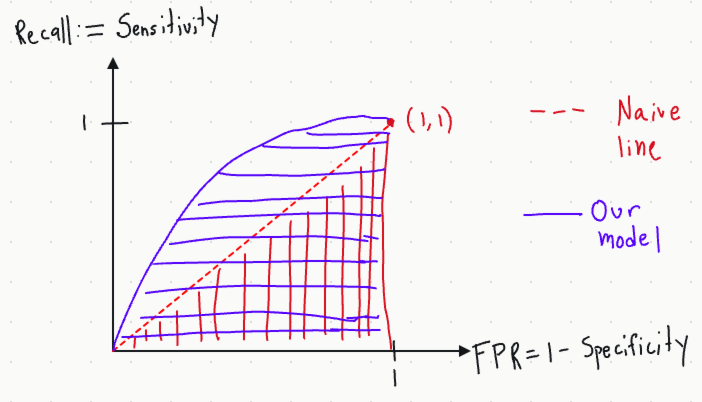
\includegraphics[width=0.7\textwidth]{receiver-operator-curve}
		\caption{The ROC curve, a plot of Recall vs. $FPR$. The dotted line is the naive
		model, and the solid line is ``our model". Each point on each curve
		corresponds to a distinct value of $p_{\text{th}}$, since both
		$FPR$ and Recall are functions of $p_{\text{th}}$.}
		\label{fig:receiver-operator-curve}
	\end{figure}
	
	Figure~\ref{fig:receiver-operator-curve} plots Recall vs. $FPR$ for
	the $g_{\text{naive}}$ with a dashed line. Each point corresponds to
	a different value of $p_{\text{th}}$ (as given by our grid). It is
	a straight line since Recall = $FPR$ for $g_{\text{naive}}$, as we
	showed. The area under the curve of $g_{\text{naive}}$ is $0.5$.
	The figure also shows a curve for a hypothetical model in a solid line.
	The area under the curve is larger than that of $g_{\text{naive}}$.
	We call this curve the \textbf{Receiver Operator Curve (ROC)}.
	The ROC allows for comparisons among probability estimation models,
	similar to the Brier and log scoring rules. It is computationally
	intensive, but some prefer it since it gives a very intuitive comparison.
	For example, if the area under the curve comes out to $0.501$, then
	the model barely outperforms picking numbers at random.
	
	\section{FDR vs. FOR}
	Let's revisit the definitions of $FDR$ and $FOR$:
	\begin{align*}
		FDR := \frac{FP}{PP} \quad\quad\quad FOR := \frac{FN}{PN}
	\end{align*}
	Note that the other error metrics are a function of $N$ and $P$,
	but that's not reality because we do not have access to these
	(we do not get to see the $y$'s). That is why $FDR$ and $FOR$
	are better (this is an opinion). So, this motivates a curve that graphs
	$FDR$ vs. $FOR$. See Figure~\ref{fig:fdr-vs-for}.
	\begin{figure}
		\centering
		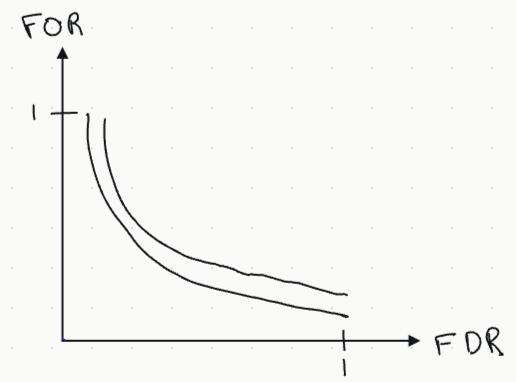
\includegraphics[width=0.5\textwidth]{fdr-vs-for}
		\caption{Comparing models by plotting FDR vs. FOR.}
		\label{fig:fdr-vs-for}
	\end{figure}
	Note the trade-off: high $FDR$ corresponds to low $FOR$, and viceversa.
	Unlike the Recall vs. $FPR$ line, there is no comparison against a
	naive line, but we can use it to compare models. It is useful for
	reading error rates, which is what we are interested in when we predict
	the future.
\end{document}